\section{Αποτελέσματα και σχολιασμός}

Στα παρακάτω σχήματα φαίνονται χαρακτηριστικές στιγμές στην εξέλιξη της ροής. Αρχικά, παραθέτουμε τη στιγμή που σχηματίζεται το πρώτο κύμα κρούσης, έπειτα το δεύτερο και τέλος την αποκατάσταση της ροής.

\begin{figure}[h!]
    \begin{center}
        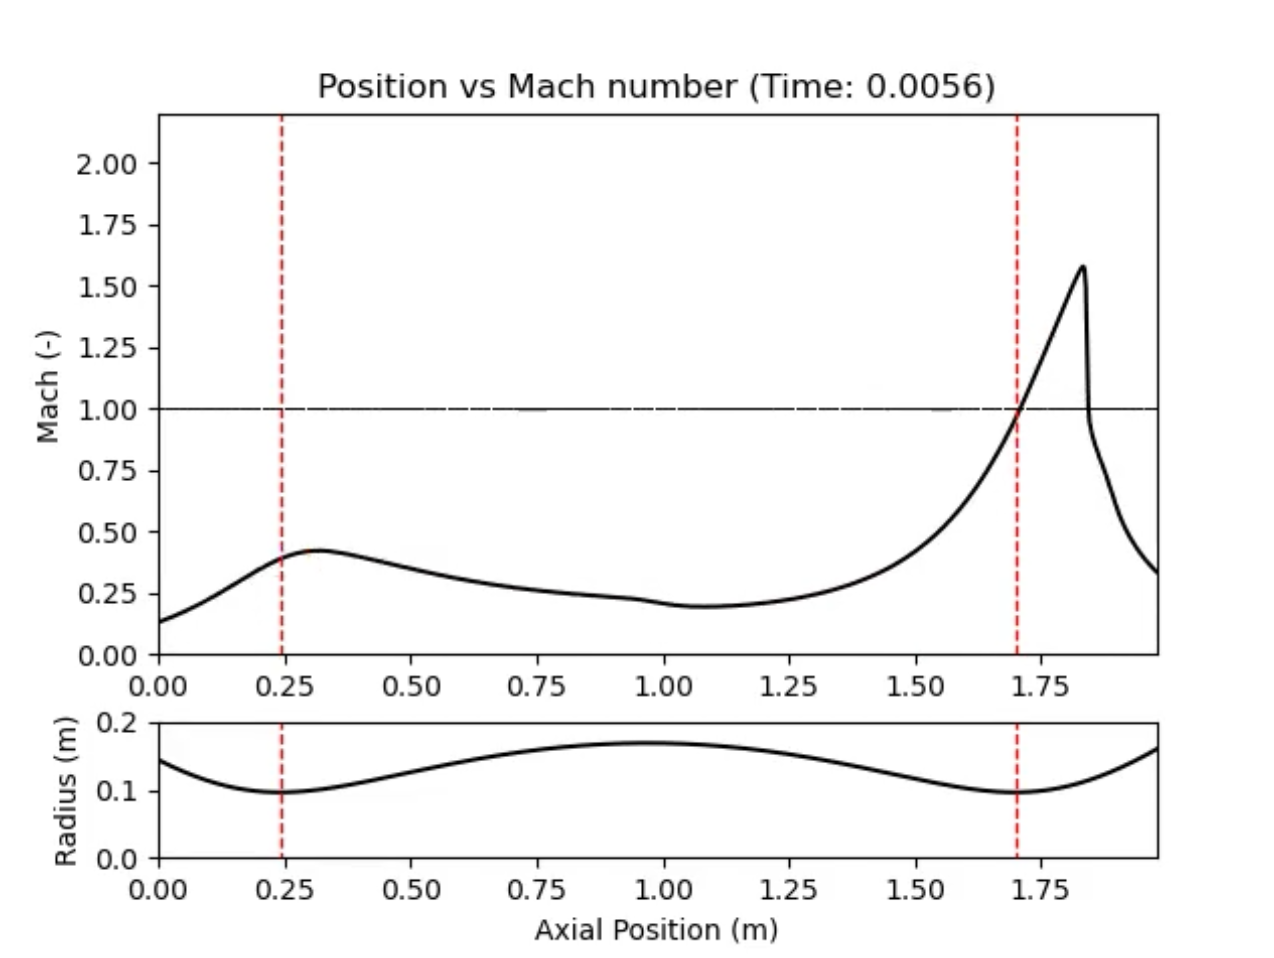
\includegraphics[width=0.85\textwidth]{figures/first_shock.png}
    \end{center}
    \caption{Σχηματισμός πρώτου κύματος κρούσης}
    \label{fig:firstshock}
\end{figure}

\begin{figure}[h!]
    \begin{center}
        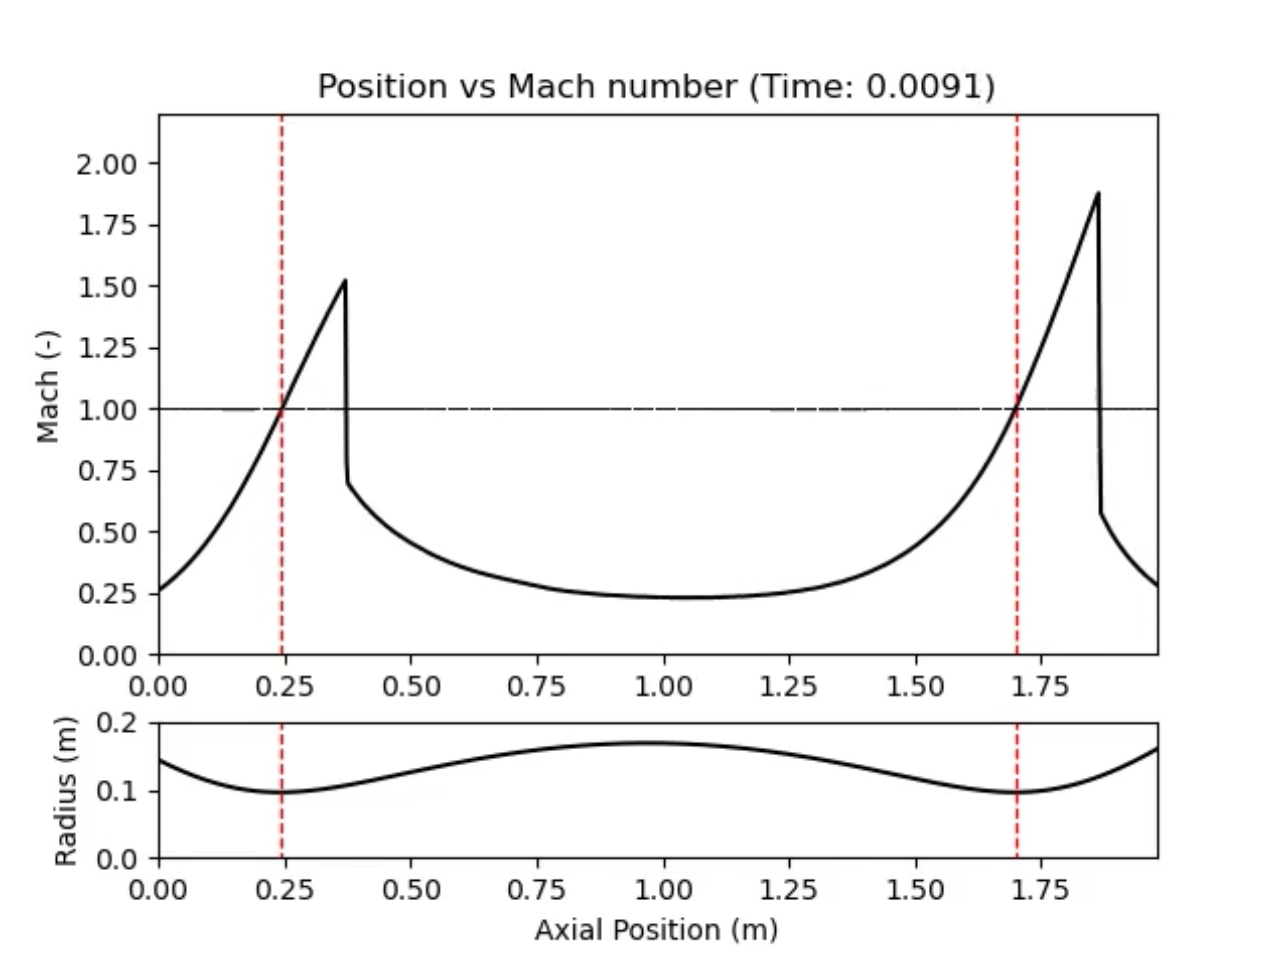
\includegraphics[width=0.85\textwidth]{figures/second_shock.png}
    \end{center}
    \caption{Σχηματισμός δεύτερου κύματος κρούσης}
    \label{fig:secondshock}
\end{figure}

\begin{figure}[h!]
    \begin{center}
        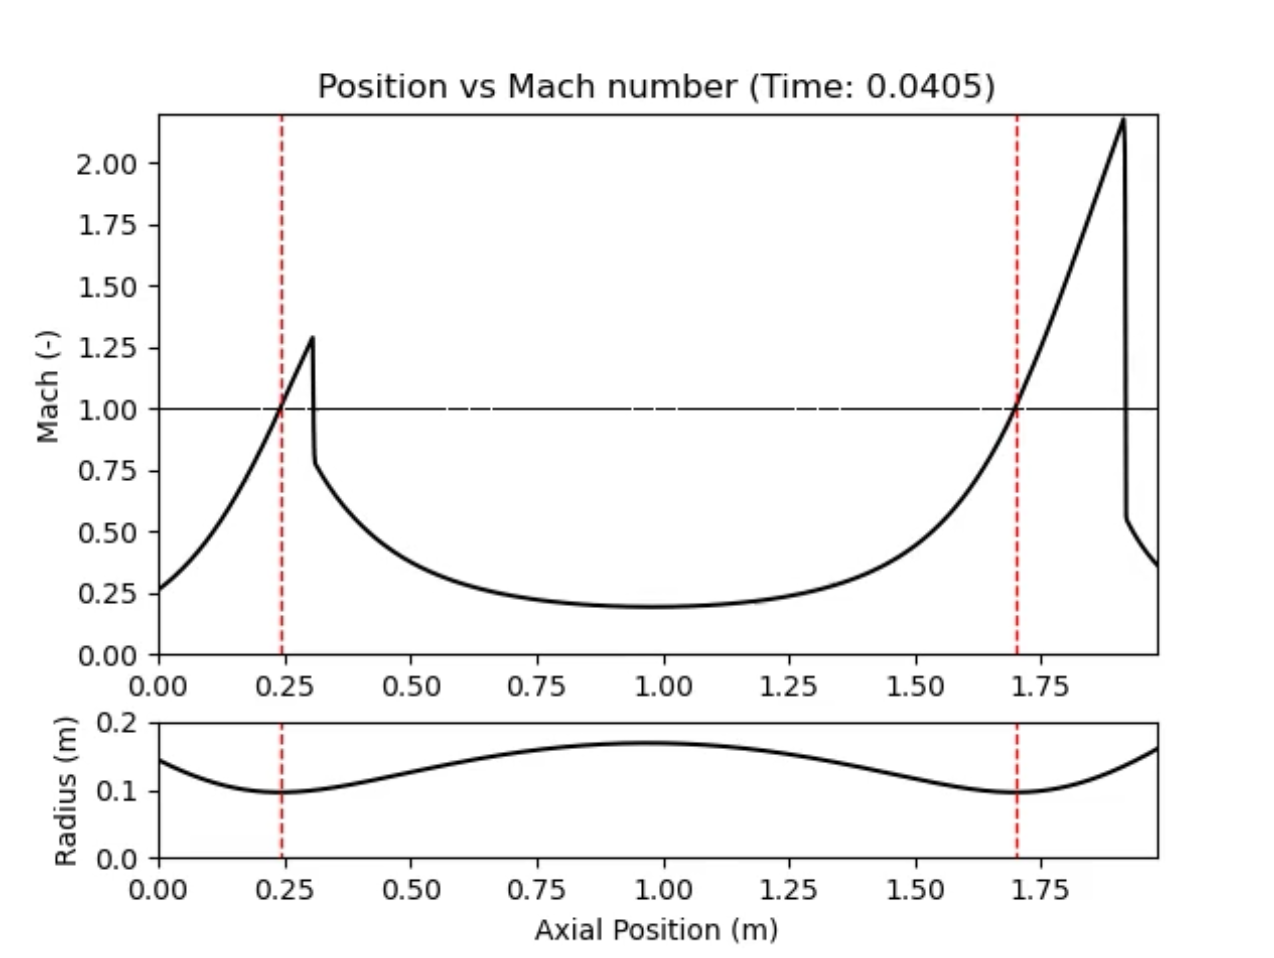
\includegraphics[width=0.85\textwidth]{figures/steady.png}
    \end{center}
    \caption{Αποκατάσταση μόνιμης ροής}
    \label{fig:steady}
\end{figure}


Απο τα στιγμιότυπα και το βίντεο της εξέλιξης της ροής παρατηρούμε πως όταν ανοίγει το αεροφυλάκιο η ροή ξεκινά απο το αεροφυλάκιο και προχωρά προς την έξοδο σαν ενα κύμα. Φαίνεται επίσης σα να αποκαθίσταται η ροή απο την έξοδο προς την είσοδο, και σχηματίζεται πρώτα το κύμα κρούσης στον δεύτερο λαιμό (κοντά στην έξοδο) όπως φαίνεται και στο σχήμα \ref{fig:firstshock} και όταν σταθεροποιείται η ροή κοντά στον δεύτερο λαιμό, αρχίζει να αποκαθίσταται και στα πίσω τμήματα. Πράγματι, στη συνέχεια εμφανίζεται και δεύτερο κύμα κρούσης μετά τον πρώτο λαιμό και η ροή αρχίζει αργά να αποκαθίσταται. 

Επιπλέον, απο όλες τις στιγμές των στιγμιότυπων στα διαγράμματα του αριθμού Mach, παρατηρούμε πως στα σημεία των λαιμών έχουμε αριθμό Mach ίσο με τη μονάδα, που συμφωνεί με τα αναμενόμενα βάσει της θεωρίας.

Τέλος, βλέπουμε πως στην αποκατεστημένη ροή μετά τον δεύτερο λαιμό έχουμε πολύ μεγαλύτερο κύμα κρούσης όπου ο αριθμός Ma ξεπερνά το 2, και απο υπερηχητική η ροή μεταβαίνει σε υποηχητική για να μεταβεί στις συνθήκες εξόδου, όπως φαίνεται και στα αντίστοιχα βίντεο με τα διαγράμματα πίεσης και πυκνότητας.

